\documentclass[a5paper]{article}
\usepackage[a5paper, top=8mm, bottom=8mm, left=8mm, right=8mm]{geometry}

\usepackage{polyglossia}
\setdefaultlanguage[babelshorthands=true]{russian}

\usepackage{fontspec}
\setmainfont{FreeSerif}
\newfontfamily{\russianfonttt}[Scale=0.7]{DejaVuSansMono}

\usepackage[font=scriptsize]{caption}

\usepackage{amsmath}
\usepackage{amssymb,amsfonts,textcomp}
\usepackage{color}
\usepackage{array}
\usepackage{hhline}
\usepackage{cite}

\usepackage[hang,multiple]{footmisc}
\renewcommand{\footnotelayout}{\raggedright}

\PassOptionsToPackage{hyphens}{url}\usepackage[xetex,linktocpage=true,plainpages=false,pdfpagelabels=false]{hyperref}
\hypersetup{colorlinks=true, linkcolor=blue, citecolor=blue, filecolor=blue, urlcolor=blue, pdftitle=1, pdfauthor=, pdfsubject=, pdfkeywords=}

\usepackage{tabu}

\usepackage{graphicx}
\usepackage{indentfirst}
\usepackage{multirow}
\usepackage{subfig}
\usepackage{footnote}
\usepackage{minted}

\sloppy
\pagestyle{plain}

\title{Лекция 1: Введение, основы F\#}

\date{18.02.2022}

\begin{document}

\maketitle
\thispagestyle{empty}

\section{О чём этот курс}

В этом семестре курс называется <<Структуры и алгоритмы компьютерной обработки данных>>, но это довольно размытое название, а заниматься мы будем последней из популярных парадигм программирования, которая ещё не была покрыта на практиках --- функциональным программированием. Речь пойдёт сначала про функциональное программирование вообще и функциональное программирование на примере языка F\#, но потом мы затронем и другие темы, используя F\# в качестве языка, такие как продвинутое многопоточное программирование, компиляторы, может быть, анализ данных и машинное обучение.

Про функциональное программирование будет рассказано немного теории (про нетипизированное лямбда-исчисление прежде всего, и про него будет всего одна пара, то есть меньше, чем про него обычно рассказывают в курсах про ФП, но у нас тут довольно вводный курс --- очень рекомендую спецкурс про ФП на 4-м курсе, или, для любителей математики, курс от Дениса Николаевича Москвина \url{https://www.lektorium.tv/course/22797}, там про лямбда-исчисление более обстоятельно и курс реально очень годный; есть ещё годные курсы от Москвина \url{https://stepik.org/course/75} и \url{https://stepik.org/course/693}, они про Хаскель, но какая разница?). Будет и много практики --- как вообще на этом программировать (без состояний, следовательно, без переменных, циклов и прочих привычных штук), про функции высших порядков, каррирование и прочие подобные вещи.

Будет отдельная пара (и, может, не одна) про типы в функциональных языках и связанные с ними вещи: чем хорошо то, что нет состояния, для реализации таких структур данных, как списки, что даёт автоматический вывод типов --- генерики, автоматическое обобщение типов функций и т.д. Будут и специфичные для функционального программирования паттерны и стили --- point-free (стиль программирования, представляющий программу как композицию функций, с явным указанием аргументов только в самом конце), Continuation Passing Style (стиль записи последовательного вычисления как цепочки функций, каждая из которых делает свою работу и вызывает <<продолжение>>), монады (или, в F\#, Computation Expressions или Workflows, способ управлять самим процессом вычисления, исполняя или не исполняя некоторые операторы в программе, выполняя какие-то действия между исполнением операторов, и т.д., при этом без дополнительного кода, if-ов и прочих вещей).

Будет и про технологические аспекты программирования на F\#, и, на самом деле, на .NET вообще. В частности, F\#, помимо того, что функциональный, ещё и объектно-ориентированный язык, со своими особенностями, о которых в этом курсе будет рассказано (кстати, совмещение объектно-ориентированного и функционального стиля даёт некоторые интересные эффекты, например, параметризация объектов функциями, что иногда может превратиться во что-то, очень похожее на полиморфизм, только гораздо гибче). Интересно то, что эти особенности постепенно переносятся в C\# и иногда даже в Java (в Java 10 таки сделали локальный автовывод типов, например). Вообще, F\#, по крайней мере, объектно-ориентированную его часть, можно рассматривать как C\# из недалёкого будущего (даже primary constructors в C\# уже вроде как реализованы и находятся в статусе experimental feature, в C\# 8 сделали switch expressions, которые в F\# назывались оператором match и были всегда, а в C\# 9 расширили pattern matching, чтобы было ещё более как в F\# --- но пока в C\# нет встроенных списков, F\# лучше). Так что знать F\# полезно не только из любви к науке, но и чтобы лучше владеть C\# (и немножко Java, Java слегка отстаёт от научно-технического прогресса, но есть Scala и Котлин --- Scala в каком-то смысле можно считать <<F\# для Java-машины со странным синтаксисом>>).

Будет немного продолжения про многопоточное программирование --- не потому, что оно связано с функциональным, а просто потому, что про него обязательно надо знать, а программа обучения на ТП устроена так, что можно счастливо избежать подробностей про него. Правда, функциональное и многопоточное программирование всё-таки хорошо уживаются вместе и дополняют друг друга: с одной стороны, чисто функциональные программы легко параллелятся, поскольку не имеют разделяемого состояния, с другой стороны, в функциональных языках есть методы управления процессом вычисления (те самые монады), которые позволяют писать многопоточные программы просто и красиво (что не отменяет возможности прострелить себе ногу, если не понимать, что происходит). В F\#, в частности, есть монада \textit{async}, которая работает так же, как ключевое слово \textit{async} в C\#, но не требует поддержки компилятора, это просто библиотечный класс.

С формальной точки зрения, для того, чтобы получить зачёт, надо будет, как в прошлом семестре, набрать достаточное количество баллов по домашкам и контрольной, которая будет где-то в середине семестра. Домашки будет довольно много, но поначалу она будет простая, чтобы дать всем возможность проникнуться духом функционального программирования и досдать долги, а потом она будет небольшая, чтобы оставить время на учебную практику, так что только одна-две домашки за весь курс будут требовать много времени. Как обычно, будет пара с докладами, за успешно сделанный доклад прощается одна домашка. Баллы за домашку, как в прошлом семестре, считаются как $MAX(0, (n/N – 0.6)) * 2.5 * 100$, баллы за контрольную: $n/N * 100$, итоговая оценка --- минимум из этих баллов. Как и в прошлом семестре, будут дедлайны по домашкам в две недели (за исключением домашки про компиляторы, она требует несколько больших усилий), за сдачу после дедлайна -0.5 за каждую пропущенную неделю (то есть за день после дедлайна -0.5, за неделю после дедлайна -1). Будут штрафы за лишние попытки (-0.5 за каждую попытку, начиная с третьей). В отличие от предыдущего семестра, в этом задачи в большинстве своём реально простые, так что пропустить дедлайн, во-первых, позорно, во-вторых, критично --- вы теряете не 0.5 балла из 15, а по 0.5 за каждую из пяти задач в домашке, тем сразу ополовинивая её стоимость. Правда, больше половины, как и в прошлом семестре, потерять нельзя.

Вот примерно какие баллы надо получить на какую оценку ECTS:
\begin{itemize}
    \item Всего около 34 баллов за д/з и по 10 за к/р
    \item A --- 33 балла за домашки, 9 за контрольную
    \item B --- 32 баллов за домашки, 8 за контрольную
    \item C --- 30 баллов за домашки, 7 за контрольную
    \item D --- 29 баллов за домашки, 6 за контрольную
    \item E --- 28 баллов за домашки, 5 за контрольную
\end{itemize}

Вполне возможно, что появятся какие-то новые домашки (например, по ML, если он таки будет), возможно, что поменяются баллы и за уже существующие задачи, вас предупредят. Как обычно, для зачёта надо набрать E. 

Этот семестр правда проще предыдущего, поскольку требования к учебным правилам более жёсткие, так что надо вас немного разгрузить.

\section{Введение в функциональное программирование}

Теперь, собственно, можно перейти к содержательной части пары. Начнём мы с главных отличий функционального программирования от того, как вы программировать привыкли.

В императивном программировании, как всем должно быть известно, программа представляет собой последовательность команд некоторому исполнителю (от непосредственно процессора, если программировать в машинных кодах, до некоторой абстрактной машины, если программировать на языках высокого уровня). Есть понятие <<состояние>>, исполнитель может, выполняя команды, модифицировать это состояние, и вся программа представляет собой постепенную модификацию состояния из начального в конечное. Естественно, бывают бесконечно работающие программы, но сути дела это не меняет --- есть некоторое начальное состояние и последовательность команд, которые в зависимости от текущего состояния могут оное состояние изменять.

Есть теорема Бёма-Якопини (\url{https://en.wikipedia.org/wiki/Structured_program_theorem}), доказанная аж в 1966 году, которая говорит о том, что любой алгоритм может быть представлен с помощью последовательного исполнения, оператора ветвления по булевому условию (обычного \textbf{if}) и цикла с булевым условием выхода (обычного \textbf{while}). Через два года после публикации работы с этой теоремой вышла знаменитая статья Э. Дейкстры <<Go To Statement Considered Harmful>>, так появилось структурное программирование. Состояние совершенно необходимо структурному программированию, потому что изменяющиеся значения переменных позволяют управлять процессом вычислений (те самые булевые условия в ветвлениях и циклах). 

Но вообще, императивное программирование появилось гораздо раньше структурного, и само понятие <<состояние>> появилось благодаря машине Тьюринга (где, как вы, должно быть, помните, была бесконечная лента и исполнитель, который управлялся в том числе и символами, записанными на ленте, при этом он мог её модифицировать). Машина Тьюринга фактически оказалась реализованной в архитектуре фон Неймана --- лента перестала быть бесконечной, схема работы с памятью стала посложнее, но принципы остались теми же. Есть ещё гарвардская архитектура, где программа и данные разделены, но она всё равно <<предрасположена>> к императивному стилю, разве что полиморфный код не позволяет писать, но его всё равно давно никто особо не пишет. Бывают и другие принципы, отличающиеся от машины Тьюринга, например, Dataflow architecture, где исполнение инструкций определяется не поведением вычислителя, а готовностью данных для инструкции, и, что интересно, современные процессоры исполняют инструкции именно по такой схеме, переупорядочивая инструкции в программе динамически, что доставляет такую боль при многопоточном программировании, но это внутреннее дело процессора, программы всё равно пишутся императивно. С компьютерами, работающими не по фон-неймановским принципам, так и не сложилось, и только относительно недавно стали популярны вычисления общего назначения на видеокартах, которые по сути представляет собой массив из сотен специализированных процессоров, имеющих каждый свою собственную и все вместе общую память, они уже достаточно сильно отличатся от классической фон-неймановской архитектуры. Долгое время ничего такого не было, поэтому императивные языки были столь популярны и, в силу большой инертности программистского и инженерного сообществ, остаются самым популярным подходом к программированию (объектно-ориентированное программирование, естественно, императивно по своей природе).

Функциональное программирование --- это очередной радикальный поворот в представлениях о программировании, потому что оно базируется на $\lambda$-исчислении Чёрча и тем самым радикально отличается от императивного программирования и вообще от концепций фон Неймана и Тьюринга. По идее, это должно вызывать некоторые страдания, но, как показывает практика, основные концепции ФП усваиваются очень неплохо (видимо, потому, что оно проще и естественнее, чем ООП). Функциональная программа --- это не более чем вычисление значения некоторой функции (в математическом смысле функции, то есть без побочных эффектов) на некоторых входных данных. В принципе, входные данные можно рассматривать как начальное состояние программы, результат --- как конечное, но промежуточных состояний в функциональных программах нет. Вообще (ну, практически).

Если функциональные программы не оперируют состоянием вычислителя, из этого следуют забавные вещи: нет состояния --- нет переменных, нет переменных --- нет циклов, нет циклов и переменных --- нет возможности задать поток управления или даже просто последовательность действий. Это могло бы быть очень печально, но раз состояния нет, то и последовательность вычислений не важна --- результат зависит только от входных данных, в каком порядке вычисляются подвыражения в программе, не важно (на самом деле, не всё так просто, но про это попозже). Забавный побочный эффект --- у чисто функциональных программ сложно с взаимодействием с пользователем, ведь даже вывод на экран --- это побочный эффект, а при условии отсутствия возможности явно управлять потоком исполнения взаимодействие с пользователем может стать весьма хаотичным. К счастью, с применением некоторого количества высшей алгебры эта проблема решается, что доказывает, например, XMonad (оконный менеджер для Linux, написанный на Haskell, \url{http://xmonad.org/}).

Простой пример различия в стиле программирования, код на C++:
\begin{minted}{c++}
int factorial(int n) {
    int result = 1;
    for (int i = 1; i <= n; ++i) {
        result *= i;
    }
    return result;
}
\end{minted}

И код на F\#:
\begin{minted}{fsharp}
let rec factorial x =
    if x = 1 then 1 else x * factorial (x - 1)
\end{minted}

Конечно, на C++ можно написать программу как на F\#, но на функциональных языках можно писать программы только так, как в примере кода для F\#-а. Никаких циклов, переменных, в которых накапливается значение, и прочих привычных штук. Однако видно, что if-ы есть (почему нет, это просто функция от трёх аргументов), рекурсия есть, возможность передавать параметры в функции есть. А это значит, что жить можно --- переменные и вообще состояние можно эмулировать, передавая в функцию параметры и возвращая модифицированные параметры (на самом деле, в функциональных языках есть структуры, так что можно в качестве параметра передавать всякие сложные штуки, хоть всё состояние программы). Циклы, естественно, делаются с помощью рекурсии, в качестве счётчика цикла можно использовать один из параметров (как было продемонстрировано в факториале), последовательность вычислений эмулируется цепочками из рекурсивных вызовов функций.

Внимательный читатель, наверное, усомнится в достаточности рекурсии для любой программы --- ведь размер стека вызовов конечен, так что рекурсивный факториал начнёт падать с переполнением стека уже при вычислении факториала от 10000. Как же тогда, например, обходить списки из 10000 элементов и вообще делать то, что делалось в императивных языках обходом в цикле большой структуры данных? Интересно, что и программа из примера выше на самом деле упадёт с переполнением стека, но есть понятие <<хвостовая рекурсия>> --- поддержка со стороны компилятора рекурсивного вызова функцией самой себя в самом конце, он такие штуки превращает в циклы. Зачем, как и как этим пользоваться, будет немного потом, сейчас важно знать, что есть простой приём программирования, который позволяет при рекурсивном вызове не использовать стек вообще, а вести себя так, будто это обычный цикл.

Вот ещё один небольшой пример, поясняющий суть дела:
\begin{minted}{fsharp}
let rec sumFirst3 ls acc i =
    if i = 3 then 
         acc 
    else 
        sumFirst3 
            (List.tail ls) 
            (acc + ls.Head) 
            (i + 1)
\end{minted}

Это, как не трудно догадаться, функция, складывающая первые три элемента в списке. Здесь, кстати, видно некоторые синтаксические особенности F\#, типичные и для других функциональных языков. Первое --- это автоматический вывод типов: аннотаций типов в программе нет, тем не менее, тип каждой <<переменной>> (не переменной, а имени на самом деле) известен во время компиляции. Второе --- рекурсивные функции объявляются с помощью ключевого слова rec, чтобы их имя было видно внутри их тела. Более по существу, здесь видно использование счётчика цикла (параметр \textit{i}) и аккумулятора (параметр \textit{acc}). Аккумулятор --- это первый паттерн функционального программирования, с которым вам придётся познакомиться, он как раз и делает хвостовую рекурсию практически полезной. 

Аккумулятор, по сути, это обычный параметр, который накапливает текущее посчитанное значение, чтобы по достижении базы рекурсии функция могла его просто вернуть. Можно было бы не использовать аккумулятор, а прибавлять ls.Head к результату рекурсивного вызова sumFirst3, но тогда \textbf{после} рекурсивного вызова пришлось бы делать операцию сложения, поэтому надо было бы хранить адрес инструкции, которую надо выполнять после рекурсивного вызова и значения параметров (рекурсивно вызвались от List.tail ls, но потом нам надо прибавить ls.Head, так что придётся хранить ls всё время), а для этого надо кадр стека вызовов. С аккумулятором дела обстоят иначе --- сложение выполняется \textbf{до} рекурсивного вызова, так что рекурсивный вызов --- это последняя операция в sumFirst3, так что при рекурсивном вызове достаточно просто присвоить новые значения параметрам и передать управление на начало функции, будто это цикл <<while>>. Никакого кадра стека для хранения чего-либо не нужно. В этом и есть суть хвостовой рекурсии, и, как мы потом увидим, в байт-код она генерируется именно так. Плохая новость в том, что компилятор F\# не умеет подсказывать, что рекурсия не хвостовая, хорошая новость в том, что хвостовая рекурсия довольно очевидна при некоторой привычке и будет получаться автоматически.

\section{Зачем нужно функциональное программирование}

Понятно, что большая часть интересных вещей в мире делается ради лулзов, но функциональные языки давно уже не относятся к эзотерическим. Хотя они пока больше распространены среди академического сообщества, многие из них активно используются и в индустрии, кроме того, идеи из функциональных языков <<просачиваются>> в привычные объектно-ориентированные. Например, лямбда-функции, одна из основ функциональных языков, появились в C\#, C++, последней сдалась Java. В том числе поэтому четвёртый семестр проги посвящён функциональному программированию --- может, вы никогда не будете программировать на F\# (что вполне вероятно), но на человека, который не в курсе, что такое лямбда-функции, замыкание, кортежи, pattern matching и т.д., даже C\#-программисты (да что там, даже Java-программисты, несмотря на отчаянную консервативность этого сообщества) будут смотреть как на идиота. Это всё можно было бы учить и на примере C\#, но надо понимать, откуда это всё взялось, на чём основано и для чего на самом деле нужно. Интересно, кстати, что C\# перенимает языковые механизмы из F\# настолько активно и бессовестно (благо их поддерживает одна компания), что F\# можно считать чем-то вроде C\# версии $n + 3$, так что к программированию на F\# можно относиться как к программированию на секретной превью-бета-версии C\# из будущего. Поэтому, кстати, для этого курса выбран F\#, а не Haskell --- можно будет не только познакомиться с ФП, но и получить ряд практически полезных в индустриальном программировании навыков.

Так вот, преимущества функционального программирования таковы.
\begin{itemize}
    \item Строгая математическая основа --- функциональные языки базируются на $\lambda$-исчислении, которое само по себе строгая формальная система, при этом достаточно простая. Императивные языки тоже формализуются с помощью машин Тьюринга, но работать с ними мало удовольствия, в чём будет возможность убедиться в курсе матлогики и потом ещё в курсе про формальные языки.
    \item Семантика программ более естественна --- для описания семантики, то есть строгого смысла императивных программ, используются, например, такие продвинутые математические механизмы, как абстрактные машины состояний, и то получается плохо. Например, семантика языка C (самого популярного по сей день в мире) так полностью и не описана, из-за чего случаются совершенно жгучие вещи (\url{http://tmpaconf.org/images/pdf/2015/Nikolay-Shilov-A-Need-To-Specify-and-Verify-Standard-Functions.pdf}). Семантика функциональных программ более очевидна.
    \begin{itemize}
        \item Применима математическая интуиция --- может быть, попрограммировав немного на F\#, вы поймёте, зачем была нужна АТЧ. Это может отпугнуть, но вообще математикой человечество занимается несколько тысячелетий, так что возможность переиспользовать хоть в какой-то степени накопленные результаты при программировании и получать от этого какие-то преимущества кажется привлекательной.
    \end{itemize}
    \item Программы проще для анализа в силу более простой семантики и меньшего количества зависимостей между их частями.
    \begin{itemize}
        \item Автоматический вывод типов.
        \item Широкие возможности для оптимизации --- чем лучше компилятор понимает программу, тем проще ему оптимально транслировать её в машинный код. Например, возможные нетривиальные зависимости по данным сильно мешают при оптимизации императивных программ, в функциональных программах таких проблем нет.
    \end{itemize}
    \item Оно более декларативно --- мы пишем в большой степени не как сделать, а что сделать. Это несколько упрощает жизнь программиста, позволяя не думать о деталях реализации, и жизнь компилятора, предоставляя ему пространство для манёвра.
    \begin{itemize}
        \item Ленивость --- если значение выражения так и не понадобится, его лучше не считать, поэтому давайте вообще не считать значение выражения, пока нас явно не попросили. Некоторые параметры функции, например, могут так и не посчитаться, даже когда функция уже отработала (это так в Haskell, в F\# из коробки всё считается как обычно, но можно попросить язык в конкретном случае считать лениво).
        \item Распараллеливание --- про это уже не раз говорилось, но ещё раз обращаю внимание --- есть программа без побочных эффектов и зависимостей по данным, состоящая большей частью из большого количества вычислений не зависящих друг от друга функций, есть видеокарты, на которых несколько сотен довольно быстрых процессоров и несколько гигов оперативки. Не так сложно сопоставить эти факты. Из коробки ничего интересного не происходит, но есть кое-что (например, \url{https://github.com/gsvgit/Brahma.FSharp}), что может помочь.
    \end{itemize}
    \item Модульность и переиспользуемость --- в объектно-ориентированных программах переиспользуемость достигается обычно на уровне классов, в функциональных --- на уровне функций и объединений функций ---- модулей. Причём, поскольку нет состояния, нет и зависимостей по данным, так что функция может быть вызвана кем угодно и когда угодно, при этом заведомо ничего не сломается. В ООП может быть невозможно использовать класс в юнит-тестах, потому что в конструкторе он запускает ядерную ракету, в чистом ФП функция не может иметь побочных эффектов, поэтому можно её использовать хоть где и как. F\#, правда, не чисто функциональный язык, так что там скорее как в ООП, но всё равно, более <<мелкозернистое>> переиспользование в совокупности с функциями высших порядков и разными функциональными паттернами позволяют писать кода меньше, а функциональности получать больше.
    \item Программы более выразительны. Прежде всего благодаря более развитой системе типов, чем в объектно-ориентированных языках и функциям высших порядков, и вообще отношению к функциям как к обычным данным. Можно писать очень красивый, короткий и переиспользуемый код.
\end{itemize}

Утверждение насчёт выразительности можно подтвердить примером. Берём наш старый пример со сложением первых трёх элементов списка:

\begin{minted}{fsharp}
let rec sumFirst3 ls acc i =
    if i = 3 then 
         acc 
    else 
        sumFirst3 
            (List.tail ls) 
            (acc + ls.Head) 
            (i + 1)
\end{minted}

Переписываем его с использованием функции fold (на C\# мы такое писали, если кто не помнит, освежите знания по википедии):

\begin{minted}{fsharp}
let sumFirst3 ls = 
    Seq.fold 
        (fun x acc -> acc + x) 
        0 
        (Seq.take 3 ls)
\end{minted}

Записываем это же самое с помощью forward pipeline operator:
\begin{minted}{fsharp}
let sumFirst3 ls = ls |> Seq.take 3 |> Seq.fold (+) 0
\end{minted}

Оный  forward pipeline operator на самом деле не более чем применяет функцию к аргументу, позволяя записывать программу в виде этакого конвейера:
\begin{minted}{fsharp}
let (|>) x f = f x
\end{minted}

А потом вспоминаем, что мы же на матмехе, и переписываем всю программу как композицию функций:

\begin{minted}{fsharp}
let sumFirst3 = Seq.take 3 >> Seq.fold (+) 0
\end{minted}

Ну или даже так:

\begin{minted}{fsharp}
    let sumFirst3 = Seq.take 3 >> Seq.sum
\end{minted}

Теперь у нас есть функция \textit{sumFirst3}, которую можно применить к списку, при этом в её определении сам список вообще не упоминается. А зачем, ведь \verb|>>| --- это просто функция, принимающая две функции и возвращающая третью, ей не нужно ничего знать про аргументы. Такой стиль программирования, без явного указания аргументов функций, называется, кстати, point-free (point --- это точка, в которой считается значение функции, терминология в ФП в основном пришла из математики, point-free --- это <<без явного указания аргумента>>). Про point-free и вообще про то, как работает кусок кода выше (например, что такое <<каррирование>>), у нас будет дальше в курсе, но вот так на F\# можно писать (это не значит, что нужно; программы в point-free-стиле быстро становятся нечитаемыми).

Вот ещё небольшой пример, возвести в квадрат и сложить все чётные числа в списке:

\begin{minted}{fsharp}
let calculate = 
    Seq.filter (fun x -> x % 2 = 0) 
    >> Seq.map (fun x -> x * x) 
    >> Seq.reduce (+)
\end{minted}

Принцип действия такой же, point-free и всё такое, но посмотрите, как естественно выглядит программа --- применили фильтр, оставив только чётные числа, возвели всё, что получилось, в квадрат, выполнили свёртку с операцией <<+>>, сложив всё, что получилось. Это не какие-то убогие циклы, как, например, в Java до появления stream-ов.

Встаёт вопрос, если всё так хорошо, то почему ещё не все пишут на функциональных языках. Причины довольно просты. Во-первых, функциональные программы не очень подходят для таких ненужных вещей, как взаимодействие с внешним миром. Это, конечно, обходится, но требует некоторых усилий и понимания, что неудобно. Во-вторых, функциональные программы, в силу большей декларативности, менее предсказуемы в плане скорости работы и потребляемой памяти. Пример проявления такой проблемы вы уже видели --- берём функцию с хвостовой рекурсией, дописываем, скажем, <<+1>> в конце, программа внезапно начинает падать или потреблять неадекватное количество ресурсов. В-третьих, что очевидно связано с <<во-вторых>>, функциональное программирование требует от программиста некоторой математической подготовки и желания думать, что хорошо в теории (программисты вообще склонны к честолюбию), но когда завтра релиз и ты осознаёшь, что всю ночь потратил, пытаясь наиболее изощрённо записать какой-нибудь кусок кода в point-free стиле так, чтобы компилятор не ругался, это печально. К тому же, у большинства программистов с математической подготовкой как раз дела не очень, не все же на матобесе учатся --- у ПИшек вот даже матфизики не будет, например.

\section{F\#}

Теперь всё-таки конкретно про F\#. F\# --- это типизированный функциональный язык для платформы .NET, появившийся в 2005 году как альтернатива C\#. Язык, в отличие от Haskell, не чисто функциональный, он допускает и объектно-ориентированное, и структурное программирование, позволяет выразить мутабельное состояние и имеет все проблемы, с этим связанные. Преимущества такого подхода к дизайну языка в том, что на F\# легко перейти с объектно-ориентированных или даже процедурных языков, он легко интегрируется с существующими объектно-ориентированными библиотеками, недостатки --- язык лишается большинства преимуществ чисто функционального подхода, например, ленивости вычислений <<из коробки>>.

На самом деле, F\# не разрабатывался с нуля, это реализация для платформы .NET несколько более старого языка OCaml (появившегося в 1996 году и использующегося с большей или меньшей активностью в научном сообществе и сейчас, например, в лаборатории языковых инструментов JetBrains), который сам на самом деле один из языков семейства ML (который появился аж в 1973). F\# настолько близок к OCaml, что его можно считать диалектом OCaml под .NET. Опытные камлисты скажут, что F\# не поддерживает ряд важных языковых особенностей OCaml, но я OCaml не знаю, так что не могу судить. Интересно, что под влиянием OCaml же создавалась и Scala --- довольно известный язык программирования под Java-платформу (кстати, распространена Scala шире, чем F\#, видимо, в силу большей популярности Java). Поэтому F\# и Scala довольно похожи, хотя Scala использует свой и очень непохожий на OCaml синтаксис. Создавались эти языки с близкими целями в примерно одно время, так что они близкие родственники, несмотря на то, что внешне непохожи.

F\# создан для платформы .NET, поэтому компилируется в её байт-код, использует её среду времени выполнения, всю инфраструктуру и даже стандартную библиотеку (хотя имеет и свою, естественно). Может работать в компилируемом режиме (как C\#) и в интерпретируемом (как, например, Python), когда программа просто исполняется построчно без компиляции. Имеется и интерактивный режим, когда пользователь может ввести выражение и тут же посчитать ответ.

F\# по сей день является несколько <<эзотерическим>> языком и довольно вяло используется в промышленной разработке. Но используется, в основном в финансовой сфере и в различного рода R\&D-проектах (в самом же Microsoft, например, или вот в Ланит-Теркоме был проект на F\#). Поскольку F\# сильно похож на Scala, F\#-разработчиков часто с удовольствием приглашают на позиции Scala-программистов, поскольку F\# работает под .NET, часто бывает так, что проекты в основном на C\# имеют некоторую часть кода, написанную на F\#-е. По данным опроса, проводимого Stack Overflow в 2016 году, F\# был самым высокооплачиваемым навыком по всемирной статистике (в 2017 году он оказался уже на 4-м месте, после Clojure, Rust и Elixir). Отчасти потому, что F\# специалистов мало и они, как правило, довольно круты. А это, в свою очередь, потому, что работу на F\# нынче найти сложновато (в Санкт-Петербурге, например, не видел ни одной вакансии).

Впрочем, функциональное программирование надо знать, даже если вы всю жизнь собираетесь проработать на Java, так что расскажу, что надо поставить, чтобы всё работало.

\begin{itemize}
    \item Visual Studio (любой её вариант, хоть Community Edition) содержит средства разработки для F\#, так что достаточно поковыряться в Visual Studio Installer, чтобы всё заработало. 
    \item Rider (для студентов он бесплатен).
    \item Visual Studio Code + .NET Core + плагин Ionide F\#, но только если вам не хочется ставить Visual Studio или она у вас тормозит, потому что Visual Studio гораздо удобнее и умнее.
    \item Первые две-три домашки можно делать без всего этого вообще, прямо в браузере: \url{https://dotnetfiddle.net/}.
\end{itemize}

\section{Пример программы}

Как обычно, изучение нового языка начинают с Hello, world. В данном случае тут всё просто:

\begin{minted}{fsharp}
printfn "%s" "Hello, world!"
\end{minted}

Сравните с кодом на C\#, который делает то же самое:

\begin{minted}{csharp}
namespace HelloWorld
{
    class Program
    {
        static void Main(string[] args)
        {
            System.Console.WriteLine("Hello, world!");
        }
    }
}
\end{minted}

(В C\# 9 тоже сделали <<скриптовый>> режим (гуглите C\# top-level statements), но совсем недавно, и если в C\# это довольно маргинальная фича, в F\# программы правда так выглядят).

Язык рассчитан в том числе и на интерпретацию, поэтому разводить всякие там классы и неймспейсы было неразумно, всё должно работать прямо так. Компилятор, на самом деле, создаст статический класс, в нём метод Main, и в нём уже тот код, что вы написали, и всё будет работать как в дотнете принято, но это более-менее скрыто от прикладного программиста, можно просто писать код.

Ну и, поскольку язык функциональный, уже встречавшийся выше пример рекурсивной функции, вычисляющей факториал:

\begin{minted}{fsharp}
let rec factorial x =
    if x = 1 then 1 else x * factorial (x - 1)
\end{minted}

Можно видеть, что в программе не упоминаются типы, хотя язык строго типизирован --- о типах заботится компилятор, выводя типы переменных (на самом деле, не совсем переменных, скорее <<имён>>, потому что они ведь не меняют значения) из их использования. Нету фигурных скобок, обозначающих границы блока --- блоки определяются отступами (как, например, в Python), отступы делаются пробелами (отступ табуляцией считается лексической ошибкой, такие дела). Нет ключевого слова return, результатом функции считается результат выражения, написанного последним (впрочем, пока мы изучаем чисто функциональное программирование, тело функции состоит из одного выражения, оно же --- её результат). Нет круглых скобок в списке формальных параметров, параметры разделяются просто пробелами (потому что каррирование, об этом чуть позже). Есть немного загадочное ключевое слово rec, которое обозначает, что factorial в теле функции надо трактовать как рекурсивный вызов, а не использование имени factorial из внешнего контекста.

\section{let-определения}

Вместо объявления переменных в F\# используются так называемые let-определения. Это что-то вроде var или auto, только let делает переменную немутабельной. Например,

\begin{minted}{fsharp}
let x = 1
let x = 2
printfn "%d" x
\end{minted}

Второе \textit{let x =} на самом деле объявляет новое имя \textit{x}, перекрывающее имя \textit{x}, объявленное ранее. И относиться к let-определению следует именно как к назначению имени некоторому выражению, то есть код выше можно читать как <<Давайте обозначим 1 за x в выражении, в котором мы обозначим 2 за x в printfn "\%d" x>>. На самом деле, в F\# есть способ записи всей этой синтаксической конструкции в одну строчку, вот так:

\begin{minted}{fsharp}
let x = 1 in let x = 2 in printfn "%d" x
\end{minted}

С математической точки зрения можно понимать let как подстановку --- компилятор заменяет то, что слева от знака равенства на то что справа в выражении, которое справа от in. На самом деле, дальше будет про лямбда-исчисление, и мы увидим, что это в точности соответствует семантике подстановки $\lambda$-терма (на самом деле внутри это работает не так, это просто объявление константы, но об этом знать пока не положено).

Функции определяются тоже через ключевое слово let, отличаются от имён они только тем, что у них есть один или более аргументов, например:

\begin{minted}{fsharp}
let powerOfFour x =
    let xSquared = x * x
    xSquared * xSquared
\end{minted}

Тут, как и в факториале с предыдущих слайдов, видно позиционный синтаксис, отсутствие return, отсутствие явных аннотаций типов, отсутствие точек с запятой (кстати, точки с запятой в F\# есть, и, как обычно, используются для определения последовательности выполнения операторов, но в чисто функциональном программировании нет такого понятия, как последовательное выполнение операторов, поэтому нам точки с запятой использовать нельзя, такие дела).

Если мы хотим функцию, которая не принимает аргументов, надо указать, что у неё один аргумент типа unit (местный аналог void):

\begin{minted}{fsharp}
let meaningOfLifeAndEverything () =
    42
\end{minted}

let-определения могут быть вложенными:
\begin{minted}{fsharp}
let powerOfFourPlusTwoTimesSix n =
    let n3 =
        let n1 = n * n
        let n2 = n1 * n1
        n2 + 2
    let n4 = n3 * 6
    n4
\end{minted}

Тут важно, что несмотря на то, что n3 использует какие-то хитрые вычисления для того, чтобы посчитать значение, это не функция, а обычная переменная. Разница в том, что функция вычисляется только когда она вызвана, а переменная получает своё значение сразу в месте определения (то есть значение n3 будет вычислено сразу, как управление дойдёт до let). Опять-таки, с точки зрения функциональной теории никакого потока управления нет, и объявление переменной --- это просто назначение имени выражению, которое её считает. А объявление функции --- это просто назначение имени выражению типа <<функция>>, которое потом можно применить к аргументам. Ещё больше может запутать дело то, что переменные вполне могут содержать функции, и бывает переменная (имя) функционального типа, а бывает функция, ведут они себя одинаково, но компилятор умеет их отличать и обрабатывает немножко по-разному. Забегая вперёд, небольшой пример:

\begin{minted}{fsharp}
let f x = x * 2
let f = fun x -> x * 2
printfn "%d" (f 5)
\end{minted}

f в первом и втором случае делает одно и то же, и работает одинаково.

\section{Типы}

Вернёмся к нашему факториалу:

\begin{minted}{fsharp}
let rec f x =
    if x = 1 then
        1
    else
        x * f (x - 1)
\end{minted}

Если его отправить в F\# Interactive (например, в Visual Studio выделить кусок кода и нажать Alt-Enter), он выдаст нам следующее:

\begin{minted}{text}
val f : x:int -> int
\end{minted}

Читать это надо как <<определено имя f типа функция, принимающая аргумент x целого типа и возвращающая целое>>. На самом деле, F\# Interactive --- очень полезный инструмент, позволяющий быстро проверить типы выражений и даже попробовать их повызывать на разных входных данных и посмотреть, как они работают. Очень рекомендую пользоваться при выполнении домашки.

На что надо обратить внимание --- тип назначается каждому имени (в том числе и функции) во время компиляции, исходя из того, как используется это имя. Здесь \textit{x} стал \textit{int}-ом просто потому, что его сравнивают с int-овым литералом и используют в операторе вычитания с int-овым литералом. Кстати, в F\# каждый литерал имеет свой тип и неявные преобразования запрещены, то есть если вы к целому прибавите беззнаковое целое --- это ошибка компиляции. Если хотите беззнаковое целое число 1, надо писать \textit{1u}.

\subsection{Элементарные типы}

Элементарные типы в языке самоочевидны и, поскольку язык на базе .NET, то отображаются в соответствующие элементарные типы .NET:

\begin{itemize}
    \item \textit{int}
    \item \textit{double}
    \item \textit{bool}
    \item \textit{string}
    \item ... (.NET). Любой дотнетовский тип, класс, перечисление и прочие подобные вещи доступны из F\#, что очень удобно, потому что можно из F\# напрямую вызывать C\#-библиотеки, и главное, пользоваться привычными типами данных, типа мутабельных списков.
    \item \textit{unit} --- тип из одного значения, (). Аналог void.
\end{itemize}

\subsection{Кортежи}

Несколько более нетрадиционный тип --- это кортежи (хотя в C\# 7 они уже появились, но вот, например, в Java даже пары ещё не изобрели). Выглядит оно как-то так:

\begin{minted}{fsharp}
let site1 = ("scholar.google.com", 10)
let site2 = ("citeseerx.ist.psu.edu", 5)
let site3 = ("scopus.com", 4)
let sites = (site1, site2, site3)

let url, relevance = site1
let site1, site2, site3 = sites
\end{minted}

Сам по себе кортеж пишется (как правило) в скобках, элементы разделяются запятой. Декомпозиция кортежа работает тоже ожидаемо, после let идёт шаблон, который пытается поматчиться структурно с кортежем справа от присваивания, и если получается, соответствующик структурные элементы присваиваются друг другу (url оказывается равен "scholar.google.com", а relevance --- 10), если не получается (например, пытаемся тройку разобрать как пару) --- ошибка компиляции. На самом деле, в let слева от равенства может стоять любой сколь угодно сложный шаблон, так что можно декомпозировать таким образом и более сложные структуры данных.

Вот кортежи, которые соответствуют Value Tuples из .NET:

\begin{minted}{fsharp}
let origin = struct (0, 0)

let displace struct (x, y) struct (dx, dy)
    = struct (x + dx, y + dy)

displace origin struct (1, 1)
\end{minted}

Синтаксически различие только в ключевом слове struct, семантически Value Tuple имеют семантику типов значений, то есть выделяются на стеке и копируются при передаче как параметры и возврате из функций, а обычные кортежи (без struct) выделяются всегда на куче и копируется только ссылка на них. Поэтому для возврата или передачи небольших кортежей, которые, к тому же, не надо долго хранить, лучше использовать value tuple, потому как reference tuple создают нагрузку на сборщик мусора.

\subsection{Функции}

Самый функциональный из всех типов --- тип-функция. Значения функционального типа удобно записывать в виде лямбда-функций, хотя и обычные функции вполне себе годятся. Лямбды используются как-то так:

\begin{minted}{fsharp}
let primes = [2; 3; 5; 7]
let primeCubes = List.map (fun n -> n * n * n) primes
\end{minted}

Если это исполнить в F\# Interactive, получится вот такое:

\begin{minted}{text}
> primeCubes;;
val it : int list = [8; 27; 125; 343]
\end{minted}

И вот ещё пример переменной, которой мы присваиваем значение типа <<функция из int в int>>:

\begin{minted}{fsharp}
let f = fun x -> x * x
let n = f 4
\end{minted}

Видно, что вызывать её можно как обычную функцию, но при этом это обычная переменная, её можно положить в список, передать как параметр и т.д. и т.п., впрочем, в любом современном языке (даже в Java) поддержка лямбда-функций есть.

\subsection{Списки}

Списки в F\# хитрее, чем вы, возможно, привыкли, они встроены в язык и, поскольку язык функциональный, немутабельны (это важно понимать, список всегда остаётся таким, каким он создан, нельзя удалить или поменять его элемент, даже добавление в голову создаёт на самом деле новый список). Вот как выглядят литералы <<спискового>> типа:

\begin{tabu} {| X[0.9 l p] | X[1 l p] | X[1 l p] |}
    \tabucline-
    Синтаксис                               & Описание                  & Пример                             \\
    \tabucline-
    \everyrow{\tabucline-}
    $[]$                                    & Пустой список             & $[]$                               \\
    $[expr; ...; expr]$                     & Список с элементами       & $[1; 2; 3]$                        \\
    $expr :: list$                          & cons, добавление в голову & $1 :: [2; 3]$                      \\
    $[expr\ ..\ expr]$                      & Промежуток целых чисел    & $[1 .. 10]$                        \\
    $[for\ x\ in\ list\ \rightarrow\ expr]$ & Генерированный список     & $[for\ x\ in\ 1..99\ \rightarrow\ x\ *\ x]$ \\
    $list\ @\ list$                         & Конкатенация              & $[1; 2]\ @\ [3; 4]$                \\
\end{tabu}

А вот пример использования списков в программе (впрочем, мы только что видели такой пример, с лямбдами):

\begin{minted}{fsharp}
let oddPrimes = [3; 5; 7; 11]
let morePrimes = [13; 17]
let primes = 2 :: (oddPrimes @ morePrimes)

let printFirst primes =
    match primes with
    | h :: t -> printfn "First prime in the list is %d" h
    | [] -> printfn "No primes found in the list"
\end{minted}

Есть одна важная проблема со списками --- значения внутри разделяются точкой с запятой, и если написать

\begin{minted}{fsharp}
let oddPrimes = [3, 5, 7, 11]
\end{minted}

--- код скомпилируется, но это будет список из одного элемента типа <<кортеж из четырёх элементов>>, такие дела. Это приносит много боли начинающим F\#-программистам, но к этому легко привыкнуть (на самом деле, это наследие OCaml, там то же самое, вроде).

Внутри списки устроены просто как пары из значения и ссылки на хвост списка. И, поскольку списки немутабельны, добавление элемента в голову --- это просто создание новой пары и установка ссылки на хвост в старый список. Например, если есть код

\begin{minted}{fsharp}
let list3 = [3; 4]
let list1 = 2 :: list3
let list2 = 1 :: list3
\end{minted}

--- получится вот такая структура в памяти:

\begin{center}
    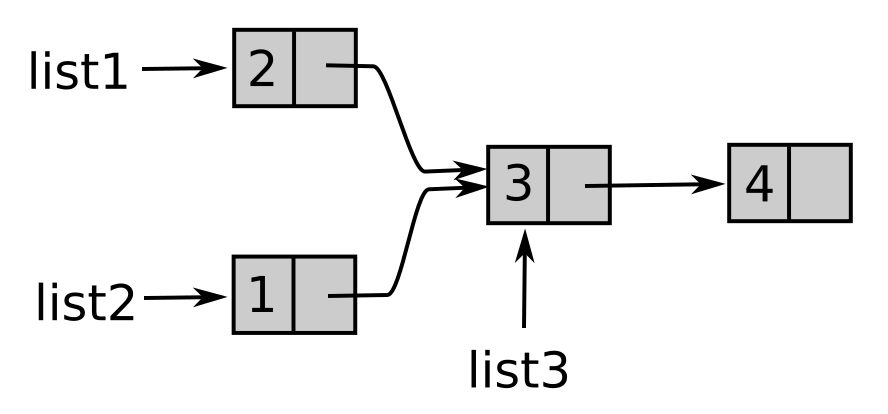
\includegraphics[width=0.5\textwidth]{lists.png}
\end{center}

Это позволяет сильно экономить память и делает операцию добавления в голову (cons) константной по трудоёмкости. Однако в конец списка добавить ничего нельзя, потому как если бы мы, например, добавили в конец list1 какой-то элемент, это добавление увидели бы list2 и list3, что нельзя, потому что списки немутабельны. Поэтому операция конкатенации копирует свой левый аргумент в новый список (а правый не копирует, кстати). Например, 

\begin{minted}{fsharp}
let list4 = list1 @ list3
\end{minted}

сделает нам новый список, у которого будут вначале копии элементов 2, 3 и 4, но элемент 4 будет ссылаться на элемент 3 из list3.

Почему списки немутабельны и как с этим жить --- это функциональный язык, тут изменяемое состояние не в почёте, и многие структуры данных реализованы так, чтобы их содержимое нельзя было менять. нет изменяемого состояния --- нет race condition-ов, нет неочевидных зависимостей по данным, можно легко менять порядок операций и т.д. и т.п. Если надо мутабельный список, всегда есть обычный дотнетовский System.Collections.Generic.List, но в первых домашках им пользоваться нельзя.

Ещё одна важная штука, отличающая F\# от более привычных, возможно, языков --- это то, что тут всякие интересные методы работы со списками вынесены в отдельный модуль. Это приём, используемый повсеместно в стандартной библиотеке --- есть какой-либо тип данных, который не умеет практически ничего и реально только хранит в себе данные, и есть отдельно класс, который содержит кучу статических методов, принимающих этот тип данных как параметр. Возможно, это кажется некрасивым с точки зрения ООП --- нарушается инкапсуляция --- но так у нас ФП. В F\# такой приём используется для того, чтобы помочь выводу типов (статический метод знает, какие типы аргументов он хочет, это сразу накладывает ограничения на используемые переменные) и для функций высших порядков, про которые чуть потом.

Со списками можно делать многое, но самое интересное в этой таблице: 
\begin{tabu} {| X[0.5 l p] | X[1 l p] | X[1 l p] | X[0.5 l p] |}
    \tabucline-
    Функция                & Описание                            & Пример                                              & Результат            \\
    \tabucline-
    \everyrow{\tabucline-}
    List.length            & Длина списка                        & $List.length\ [1;2;3]$                              & $3$                  \\
    List.nth               & n-ый элемент списка                 & $List.nth\ [1; 2; 3]\ 1$                            & $2$                  \\
    List.init              & Генерирует список                   & $List.init\ 3 (fun\ i\ \rightarrow\ i * i)$         & $[0; 1; 4]$          \\
    List.head              & Голова списка                       & $List.head\ [1; 2; 3]$                              & $1$                  \\
    List.tail              & Хвост списка                        & $List.tail\ [1; 2; 3]$                              & $[2; 3]$             \\
    List.map               & Применяет функцию ко всем элементам & $List.map\ (fun\ i\ \rightarrow\ i * i)\ [1; 2; 3]$ & $[1; 4; 9]$          \\
    List.filter            & Отбирает нужные элементы            & $List.filter\ (fun\ x\ \rightarrow\ x\ \%\ 2 <> 0)\ [1; 2; 3]$ & $[1; 3]$  \\
    List.fold              & "Свёртка"  & $List.fold\ (fun\ x\ acc\ \rightarrow\ acc * x)\ 1\ [1; 2; 3]$               & $6$                  \\
    List.zip               & Делает из двух списков список пар   & $List.zip\ [1; 2]\ [3; 4]$                          & $[(1, 3); (2, 4)]$   \\
\end{tabu}

Вообще, подробности в MSDN (\url{https://msdn.microsoft.com/visualfsharpdocs/conceptual/collections.list-module-\%5bfsharp\%5d}), старательно объяснять каждую функцию тут не будем, к тому же, они так или иначе знакомы по другим языкам (в C\# они называются немного по-другому, правда, но суть такая же).

\subsection{Option}

Следующий важный тип, который потихоньку проникает в более традиционные языки --- это Option --- абстракция наличия либо отсутствия значения. Вот небольшой пример:

\begin{minted}{fsharp}
let people = [ ("Adam", None); ("Eve" , None);
    ("Cain", Some("Adam","Eve"));
    ("Abel", Some("Adam","Eve")) ]
\end{minted}

У Адама и Евы не было родителей, поэтому их родители обозначаются None, у Каина и Авеля родители были, поэтому они Some что-то. Вообще, Option это либо Some <какое-то значение>, либо None, поскольку Option генерик, то значение может быть любого типа (хоть список чего-нибудь ужасного). Вот пример использования:

\begin{minted}{fsharp}
let showParents (name, parents) =
    match parents with
    | Some(dad, mum) -> 
        printfn "%s, father %s, mother %s" name dad mum
    | None -> printfn "%s has no parents!" name
\end{minted}

\section{Функции}

Теперь немного подробнее про функции в F\#. Рекурсию мы уже видели:

\begin{minted}{fsharp}
let rec length l =
    match l with
    | [] -> 0
    | h :: t -> 1 + length t
\end{minted}

Но в F\# компилятор не допускает использования ещё не определённых имён (в отличие от C\#, где вполне можно вызывать метод, объявленный ниже), поэтому могут наступить проблемы с взаимной рекурсией. Собственно, взаимная рекурсия --- это плохо, она запутывает поток управления, но если очень надо, то взаимно рекурсивные функции надо описать рядом через ключевое слово and:

\begin{minted}{fsharp}
let rec even n = (n = 0u) || odd(n - 1u)
and odd n = (n <> 0u) && even(n - 1u)
\end{minted}

Обратите внимание на суффиксы \textit{u} у чисел --- это обозначение беззнакового целого литерала (просто 1 был бы знаковым int-ом).

\end{document}
